\documentclass[]{article}
\usepackage[left=1in,top=1in,right=1in,bottom=1in]{geometry}
\newcommand*{\authorfont}{\fontfamily{phv}\selectfont}
\usepackage{lmodern}


  \usepackage[T1]{fontenc}
  \usepackage[utf8]{inputenc}



\usepackage{abstract}
\renewcommand{\abstractname}{}    % clear the title
\renewcommand{\absnamepos}{empty} % originally center

\renewenvironment{abstract}
 {{%
    \setlength{\leftmargin}{0mm}
    \setlength{\rightmargin}{\leftmargin}%
  }%
  \relax}
 {\endlist}

\makeatletter
\def\@maketitle{%
  \newpage
%  \null
%  \vskip 2em%
%  \begin{center}%
  \let \footnote \thanks
    {\fontsize{18}{20}\selectfont\raggedright  \setlength{\parindent}{0pt} \@title \par}%
}
%\fi
\makeatother




\setcounter{secnumdepth}{0}



\title{Ghassemi Report }
 



\author{}


\date{}

\usepackage{titlesec}

\titleformat*{\section}{\normalsize\bfseries}
\titleformat*{\subsection}{\normalsize\itshape}
\titleformat*{\subsubsection}{\normalsize\itshape}
\titleformat*{\paragraph}{\normalsize\itshape}
\titleformat*{\subparagraph}{\normalsize\itshape}

\newcommand{\dummy}[1]{#1}

\usepackage{natbib}
\bibpunct{(}{)}{;}{a}{}{,}
\bibliographystyle{plainnat}
%\usepackage[strings]{underscore} % protect underscores in most circumstances



\newtheorem{hypothesis}{Hypothesis}
\usepackage{setspace}

\makeatletter
\@ifpackageloaded{hyperref}{}{%
\ifxetex
  \PassOptionsToPackage{hyphens}{url}\usepackage[setpagesize=false, % page size defined by xetex
              unicode=false, % unicode breaks when used with xetex
              xetex]{hyperref}
\else
  \PassOptionsToPackage{hyphens}{url}\usepackage[unicode=true]{hyperref}
\fi
}

\@ifpackageloaded{color}{
    \PassOptionsToPackage{usenames,dvipsnames}{color}
}{%
    \usepackage[usenames,dvipsnames]{color}
}
\makeatother
\hypersetup{breaklinks=true,
%            bookmarks=true,
            pdfauthor={},
             pdfkeywords = {},  
            pdftitle={Ghassemi Report},
            colorlinks=true,
            citecolor=blue,
            urlcolor=blue,
            linkcolor=magenta,
            pdfborder={0 0 0}}
\urlstyle{same}  % don't use monospace font for urls

% set default figure placement to htbp
\makeatletter
\def\fps@figure{htbp}
\makeatother

\usepackage{graphicx}
\usepackage{booktabs}
\usepackage{longtable}
\usepackage{array}
\usepackage{multirow}
\usepackage{wrapfig}
\usepackage{float}
\usepackage{colortbl}
\usepackage{pdflscape}
\usepackage{tabu}
\usepackage{threeparttable}
\usepackage{threeparttablex}
\usepackage[normalem]{ulem}
\usepackage{makecell}
\usepackage{xcolor}


% add tightlist ----------
\providecommand{\tightlist}{%
\setlength{\itemsep}{0pt}\setlength{\parskip}{0pt}}

\begin{document}
	
% \pagenumbering{arabic}% resets `page` counter to 1 
%    

% \maketitle

{% \usefont{T1}{pnc}{m}{n}
\setlength{\parindent}{0pt}
\thispagestyle{plain}
{\fontsize{18}{20}\selectfont\raggedright 
\maketitle  % title \par  

}

{
   \vskip 13.5pt\relax \normalsize\fontsize{11}{12} 
 

}

}






\vskip 6.5pt


\noindent  \hypertarget{introduction}{%
\section{Introduction}\label{introduction}}

The samples studied in this report, the numbers of sequence reads,
recovered integration vectors, and unique integration sites available
for this subject are shown below. We quantify population clone diversity
using Gini coefficients, Shannon index, and UC50. The Gini coefficient
provides a measure of inequality in clonal abundance in each sample. The
coefficient equals zero when all sites are equally abundant (polyclonal)
and increases as fewer sites account for more of the total
(oligoclonal). Shannon index is another widely used measure of diversity
and it accounts for both abundance and evenness of the integration
events. Alternatively, the UC50 is the number of unique clones which
make up the top 50\% of the sample's abundance. For polyclonal samples,
one may expect a low Gini coefficient, high Shannon Index, and high UC50
(proportional to the total number of unique sites identified in the
sample).

Under most circumstances only a subset of sites will be sampled. We thus
include an estimate of sample size based on frequency of isolation
information from the SonicLength method \citet{berry2012}. The `S.chao1'
column denotes the estimated lower bound for population size derived
using Chao estimate \citet{chao1987}. If sample replicates were present
then estimates were subjected to jackknife bias correction.

We estimate the numbers of cell clones sampled using the SonicLength
method \citet{berry2012}; this is summarized in the column ``Inferred
cells''. Integration sites were recovered using ligation mediated PCR
after random fragmentation of genomic DNA, which reduces recovery biases
compared with restriction enzyme cleavage. Relative abundance was not
measured from read counts, which are known to be inaccurate, but from
marks introduced into DNA specimens prior to PCR amplification using the
SonicLength method \citet{berry2012}.

We quantify population diversity using Gini coefficients, Shannon index,
and UC50. The Gini coefficient provides a measure of inequality in
clonal abundance in each sample. The coefficient equals zero when all
sites are equally abundant (polyclonal) and increases as fewer sites
account for more of the total (oligoclonal). Shannon index is another
widely used measure of diversity and it accounts for both abundance and
evenness of the integration events. UC50 is the number of clones which
make up the top 50\% of the sample's abundance. For polyclonal samples,
one may expect a low Gini coefficient, high Shannon Index, and high UC50
(proportional to the total number of unique sites identified in the
sample).

Integration positions are reported with the format (nearest gene,
chromosome, +/-, genomic position) where the nearest gene is the nearest
transcriptional boundary to the integration position, `+' refers to
integration in the positive orientation and `-' refers to integration in
the reverse orientation. Reported distances are signed where where the
sign indicates if integrations are upstream (-) or downstream (+, no
sign) of the nearest gene. Nearest genes possess additional annotations
described in the table below.

\begin{table}[ht]
\centering
\begin{tabular}{ll}
  \hline
Symbol & Meaning \\ 
  \hline
* & site is within a transcription unit \\ 
  \~{} & site is within 50kb of a cancer related gene \\ 
  ! & nearest gene was assocaited with lymphoma in humans \\ 
   \hline
\end{tabular}
\end{table}

\hypertarget{samples}{%
\section{Samples}\label{samples}}

\begin{table}[H]
\centering
\resizebox{\linewidth}{!}{
\begin{tabular}{lllllllllll}
\toprule
GTSP & Timepoint & CellType & TotalReads & InferredCells & UniqueSites & Gini & Chao1 & Shannon & Pielou & UC50\\
\midrule
\cellcolor{gray!6}{GTSP3801} & \cellcolor{gray!6}{D7.1} & \cellcolor{gray!6}{T-Cells} & \cellcolor{gray!6}{445,904} & \cellcolor{gray!6}{444} & \cellcolor{gray!6}{314} & \cellcolor{gray!6}{0.244} & \cellcolor{gray!6}{981} & \cellcolor{gray!6}{5.60} & \cellcolor{gray!6}{0.974} & \cellcolor{gray!6}{93}\\
GTSP3802 & D7.2 & T-Cells & 569,295 & 347 & 285 & 0.165 & 2,293 & 5.53 & 0.979 & 112\\
\cellcolor{gray!6}{GTSP3803} & \cellcolor{gray!6}{D7.3} & \cellcolor{gray!6}{T-Cells} & \cellcolor{gray!6}{313,069} & \cellcolor{gray!6}{240} & \cellcolor{gray!6}{162} & \cellcolor{gray!6}{0.263} & \cellcolor{gray!6}{467} & \cellcolor{gray!6}{4.93} & \cellcolor{gray!6}{0.969} & \cellcolor{gray!6}{43}\\
GTSP3798 & D9.1 & T-Cells & 1,235,174 & 639 & 451 & 0.247 & 1,672 & 5.96 & 0.975 & 132\\
\cellcolor{gray!6}{GTSP3799} & \cellcolor{gray!6}{D9.2} & \cellcolor{gray!6}{T-Cells} & \cellcolor{gray!6}{1,303,789} & \cellcolor{gray!6}{11,765} & \cellcolor{gray!6}{11,168} & \cellcolor{gray!6}{0.049} & \cellcolor{gray!6}{129,421} & \cellcolor{gray!6}{9.30} & \cellcolor{gray!6}{0.998} & \cellcolor{gray!6}{5,286}\\
\addlinespace
GTSP3800 & D9.3 & T-Cells & 1,341,729 & 7,895 & 6,644 & 0.135 & 22,310 & 8.74 & 0.994 & 2,697\\
\bottomrule
\end{tabular}}
\end{table}

\hypertarget{relative-abundance-of-cell-clones}{%
\section{Relative abundance of cell
clones}\label{relative-abundance-of-cell-clones}}

The relative abundances of cell clones is summarized in the stacked bar
plots below. The cell fraction studied is named at the top of each plot
and the time points are marked at the bottom. The different bars in each
panel show the major cell clones, as marked by integration sites where
the x-axis indicates time points and the y-axis is scaled by proportion
of the total cells sampled. The top 10 most abundant clones from each
cell type have been named by the nearest gene while the remaining sites
are binned as low abundance (LowAbund; grey). The total number of
genomic fragments used to identify integration sites are listed atop of
each plot.

\begin{center}\includegraphics{report_files/figure-latex/abundant-1} \end{center}

\newpage

\hypertarget{scan-stats}{%
\section{Scan stats}\label{scan-stats}}

We performed a Scan Statistics analysis as described in
\citet{berry2014}. This method looks for clusters of insertion sites
that differentiate two samples in a way that prevents doing multiple
comparisons and reducing the significance of the test. Genes associated
with the Scan intervals were retrieved using two methods. genesIntsites
uses the closest gene to each insertion site. genesEntrez retrieve all
genes from the Entrez database that intersects that interval. Those
tables are also available in ``Scan\_stats.xlsx''.

\begin{table}[H]

\caption{\label{tab:scan_table}scan statistics}
\centering
\resizebox{\linewidth}{!}{
\begin{tabular}[t]{llllrrrlll}
\toprule
seqnames & start & end & width & countD7 & countD9 & target.min & clusterSource & genesIntsites & genesEntrez\\
\midrule
\cellcolor{gray!6}{chr3} & \cellcolor{gray!6}{197,977,521} & \cellcolor{gray!6}{198,005,211} & \cellcolor{gray!6}{27,691} & \cellcolor{gray!6}{6} & \cellcolor{gray!6}{1} & \cellcolor{gray!6}{0.0000772} & \cellcolor{gray!6}{D7} & \cellcolor{gray!6}{LMLN} & \cellcolor{gray!6}{LMLN}\\
chr9 & 43,401,923 & 43,447,894 & 45,972 & 4 & 0 & 0.0483634 & D7 & XLOC\_007697 & LOC105379443\\
\cellcolor{gray!6}{chr12} & \cellcolor{gray!6}{132,653,197} & \cellcolor{gray!6}{132,654,034} & \cellcolor{gray!6}{838} & \cellcolor{gray!6}{3} & \cellcolor{gray!6}{1} & \cellcolor{gray!6}{4.6910002} & \cellcolor{gray!6}{D7} & \cellcolor{gray!6}{POLE} & \cellcolor{gray!6}{POLE}\\
chr19 & 47,504,800 & 47,575,928 & 71,129 & 3 & 1 & 4.6910002 & D7 & ZNF541 NAPA & NAPA ZNF541\\
\cellcolor{gray!6}{chr22} & \cellcolor{gray!6}{50,391,250} & \cellcolor{gray!6}{50,461,381} & \cellcolor{gray!6}{70,132} & \cellcolor{gray!6}{7} & \cellcolor{gray!6}{14} & \cellcolor{gray!6}{0.6426809} & \cellcolor{gray!6}{D9} & \cellcolor{gray!6}{PPP6R2 SBF1} & \cellcolor{gray!6}{SBF1 PPP6R2}\\
\bottomrule
\end{tabular}}
\end{table}

\newpage

\hypertarget{hot-rocs}{%
\section{hot ROCs}\label{hot-rocs}}

The ROC curve heatmaps were generated as described in \citet{berry2014}.
They show how much the distribution of insertion sites across several
genomic and epigenomic features differs from a random distribution. The
heatmaps include D7 and D9 samples as well as some preinfusion samples
from \citet{nobles2020}. All samples fallow roughly the same pattern for
all features.

\begin{figure}[H]

{\centering 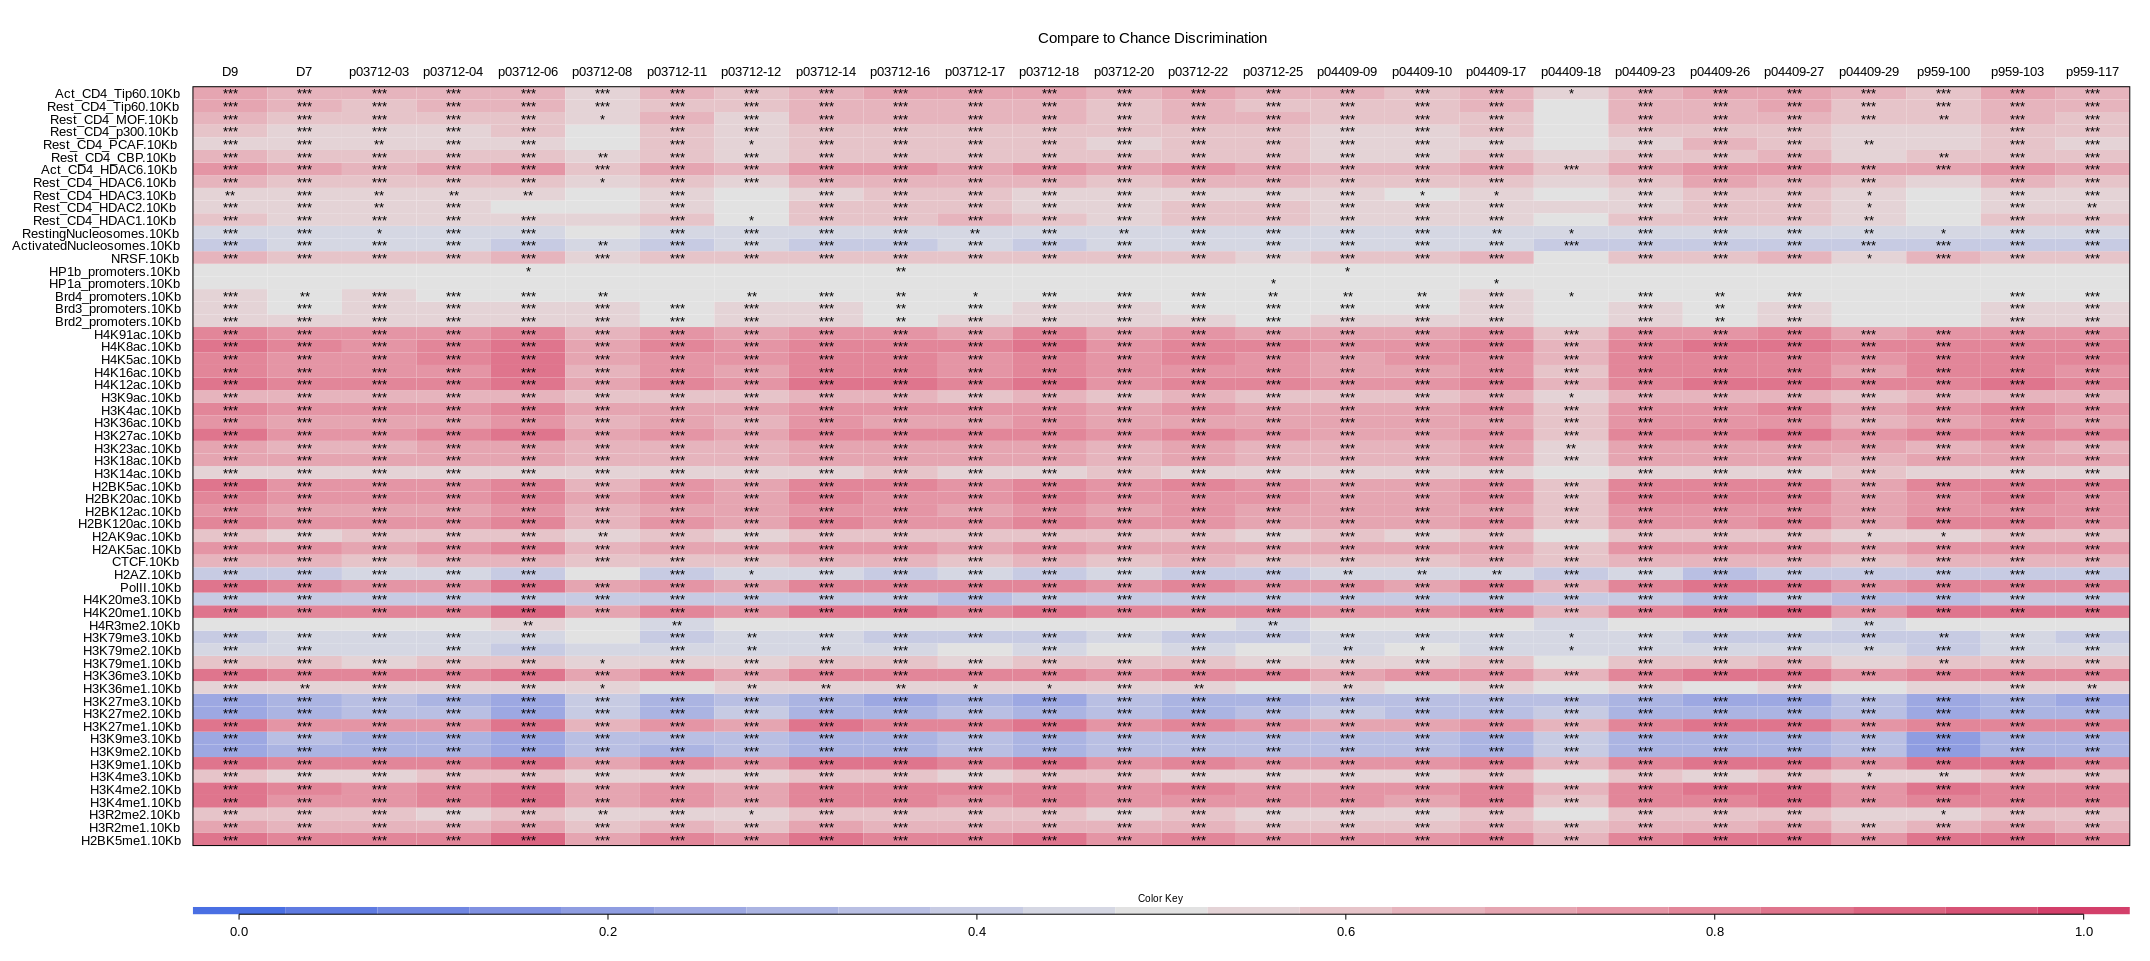
\includegraphics[width=1\linewidth]{epiGenHeatMap_ddd/main} 

}

\caption{Metagenomic features}\label{fig:unnamed-chunk-2}
\end{figure}

\begin{figure}[H]

{\centering 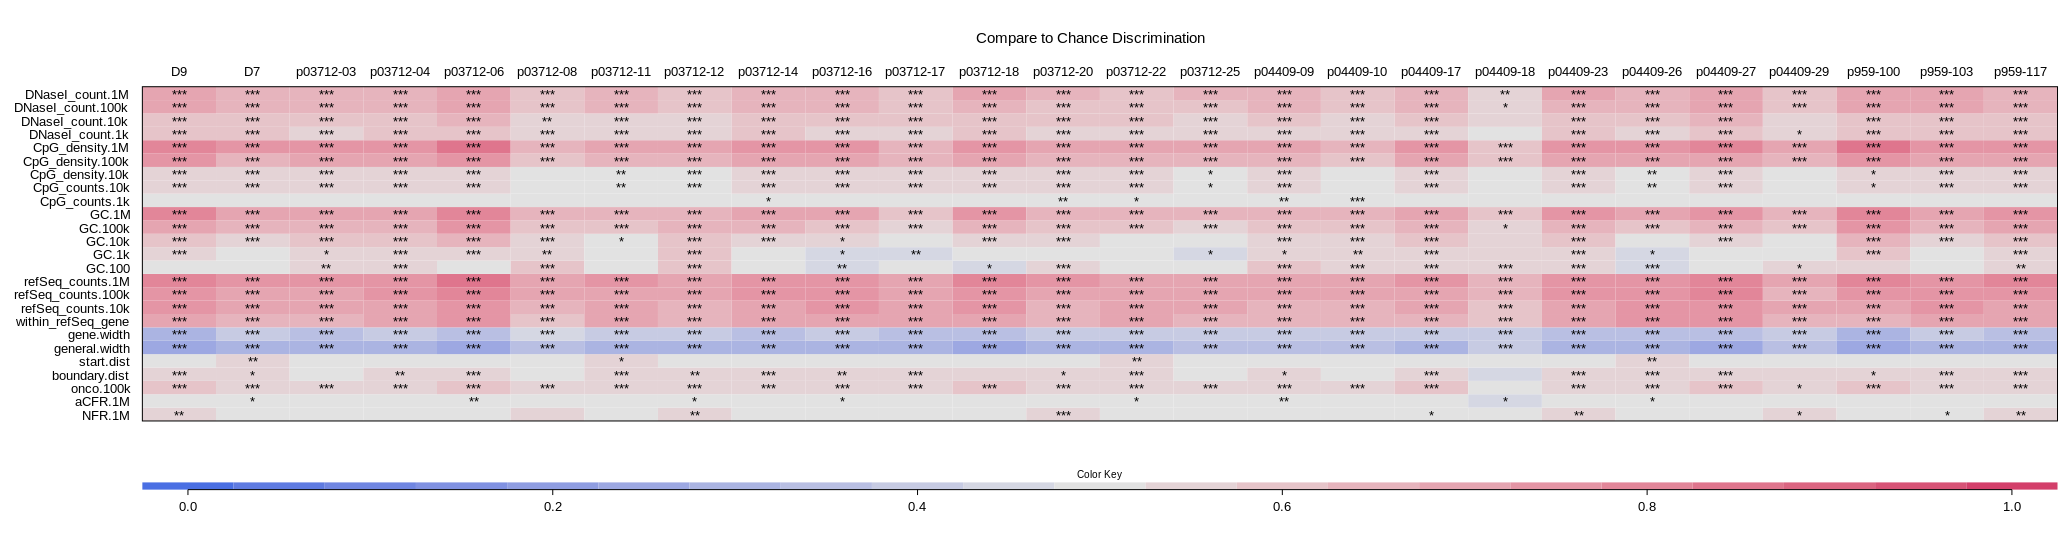
\includegraphics[width=1\linewidth]{genHeatMap_ddd/main} 

}

\caption{Genomic features}\label{fig:unnamed-chunk-3}
\end{figure}
\newpage

\hypertarget{tracking-of-clonal-abundances}{%
\section{Tracking of clonal
abundances}\label{tracking-of-clonal-abundances}}

\newpage

\hypertarget{code-availability}{%
\section{code availability}\label{code-availability}}

all the code used to generate this report is available at
\url{https://github.com/Adrian-Cantu/Ghassemi_CART}




\newpage
\singlespacing 
\bibliography{therapy.bib}

\end{document}